\documentclass[]{article}
\usepackage{lmodern}
\usepackage{amssymb,amsmath}
\usepackage{ifxetex,ifluatex}
\usepackage{fixltx2e} % provides \textsubscript
\ifnum 0\ifxetex 1\fi\ifluatex 1\fi=0 % if pdftex
  \usepackage[T1]{fontenc}
  \usepackage[utf8]{inputenc}
\else % if luatex or xelatex
  \ifxetex
    \usepackage{mathspec}
  \else
    \usepackage{fontspec}
  \fi
  \defaultfontfeatures{Ligatures=TeX,Scale=MatchLowercase}
\fi
% use upquote if available, for straight quotes in verbatim environments
\IfFileExists{upquote.sty}{\usepackage{upquote}}{}
% use microtype if available
\IfFileExists{microtype.sty}{%
\usepackage{microtype}
\UseMicrotypeSet[protrusion]{basicmath} % disable protrusion for tt fonts
}{}
\usepackage[margin=1in]{geometry}
\usepackage{hyperref}
\hypersetup{unicode=true,
            pdftitle={Business Statistics with R: Payday Loan study case},
            pdfauthor={Gibran Makyanie},
            pdfborder={0 0 0},
            breaklinks=true}
\urlstyle{same}  % don't use monospace font for urls
\usepackage{color}
\usepackage{fancyvrb}
\newcommand{\VerbBar}{|}
\newcommand{\VERB}{\Verb[commandchars=\\\{\}]}
\DefineVerbatimEnvironment{Highlighting}{Verbatim}{commandchars=\\\{\}}
% Add ',fontsize=\small' for more characters per line
\usepackage{framed}
\definecolor{shadecolor}{RGB}{248,248,248}
\newenvironment{Shaded}{\begin{snugshade}}{\end{snugshade}}
\newcommand{\AlertTok}[1]{\textcolor[rgb]{0.94,0.16,0.16}{#1}}
\newcommand{\AnnotationTok}[1]{\textcolor[rgb]{0.56,0.35,0.01}{\textbf{\textit{#1}}}}
\newcommand{\AttributeTok}[1]{\textcolor[rgb]{0.77,0.63,0.00}{#1}}
\newcommand{\BaseNTok}[1]{\textcolor[rgb]{0.00,0.00,0.81}{#1}}
\newcommand{\BuiltInTok}[1]{#1}
\newcommand{\CharTok}[1]{\textcolor[rgb]{0.31,0.60,0.02}{#1}}
\newcommand{\CommentTok}[1]{\textcolor[rgb]{0.56,0.35,0.01}{\textit{#1}}}
\newcommand{\CommentVarTok}[1]{\textcolor[rgb]{0.56,0.35,0.01}{\textbf{\textit{#1}}}}
\newcommand{\ConstantTok}[1]{\textcolor[rgb]{0.00,0.00,0.00}{#1}}
\newcommand{\ControlFlowTok}[1]{\textcolor[rgb]{0.13,0.29,0.53}{\textbf{#1}}}
\newcommand{\DataTypeTok}[1]{\textcolor[rgb]{0.13,0.29,0.53}{#1}}
\newcommand{\DecValTok}[1]{\textcolor[rgb]{0.00,0.00,0.81}{#1}}
\newcommand{\DocumentationTok}[1]{\textcolor[rgb]{0.56,0.35,0.01}{\textbf{\textit{#1}}}}
\newcommand{\ErrorTok}[1]{\textcolor[rgb]{0.64,0.00,0.00}{\textbf{#1}}}
\newcommand{\ExtensionTok}[1]{#1}
\newcommand{\FloatTok}[1]{\textcolor[rgb]{0.00,0.00,0.81}{#1}}
\newcommand{\FunctionTok}[1]{\textcolor[rgb]{0.00,0.00,0.00}{#1}}
\newcommand{\ImportTok}[1]{#1}
\newcommand{\InformationTok}[1]{\textcolor[rgb]{0.56,0.35,0.01}{\textbf{\textit{#1}}}}
\newcommand{\KeywordTok}[1]{\textcolor[rgb]{0.13,0.29,0.53}{\textbf{#1}}}
\newcommand{\NormalTok}[1]{#1}
\newcommand{\OperatorTok}[1]{\textcolor[rgb]{0.81,0.36,0.00}{\textbf{#1}}}
\newcommand{\OtherTok}[1]{\textcolor[rgb]{0.56,0.35,0.01}{#1}}
\newcommand{\PreprocessorTok}[1]{\textcolor[rgb]{0.56,0.35,0.01}{\textit{#1}}}
\newcommand{\RegionMarkerTok}[1]{#1}
\newcommand{\SpecialCharTok}[1]{\textcolor[rgb]{0.00,0.00,0.00}{#1}}
\newcommand{\SpecialStringTok}[1]{\textcolor[rgb]{0.31,0.60,0.02}{#1}}
\newcommand{\StringTok}[1]{\textcolor[rgb]{0.31,0.60,0.02}{#1}}
\newcommand{\VariableTok}[1]{\textcolor[rgb]{0.00,0.00,0.00}{#1}}
\newcommand{\VerbatimStringTok}[1]{\textcolor[rgb]{0.31,0.60,0.02}{#1}}
\newcommand{\WarningTok}[1]{\textcolor[rgb]{0.56,0.35,0.01}{\textbf{\textit{#1}}}}
\usepackage{longtable,booktabs}
\usepackage{graphicx,grffile}
\makeatletter
\def\maxwidth{\ifdim\Gin@nat@width>\linewidth\linewidth\else\Gin@nat@width\fi}
\def\maxheight{\ifdim\Gin@nat@height>\textheight\textheight\else\Gin@nat@height\fi}
\makeatother
% Scale images if necessary, so that they will not overflow the page
% margins by default, and it is still possible to overwrite the defaults
% using explicit options in \includegraphics[width, height, ...]{}
\setkeys{Gin}{width=\maxwidth,height=\maxheight,keepaspectratio}
\IfFileExists{parskip.sty}{%
\usepackage{parskip}
}{% else
\setlength{\parindent}{0pt}
\setlength{\parskip}{6pt plus 2pt minus 1pt}
}
\setlength{\emergencystretch}{3em}  % prevent overfull lines
\providecommand{\tightlist}{%
  \setlength{\itemsep}{0pt}\setlength{\parskip}{0pt}}
\setcounter{secnumdepth}{0}
% Redefines (sub)paragraphs to behave more like sections
\ifx\paragraph\undefined\else
\let\oldparagraph\paragraph
\renewcommand{\paragraph}[1]{\oldparagraph{#1}\mbox{}}
\fi
\ifx\subparagraph\undefined\else
\let\oldsubparagraph\subparagraph
\renewcommand{\subparagraph}[1]{\oldsubparagraph{#1}\mbox{}}
\fi

%%% Use protect on footnotes to avoid problems with footnotes in titles
\let\rmarkdownfootnote\footnote%
\def\footnote{\protect\rmarkdownfootnote}

%%% Change title format to be more compact
\usepackage{titling}

% Create subtitle command for use in maketitle
\providecommand{\subtitle}[1]{
  \posttitle{
    \begin{center}\large#1\end{center}
    }
}

\setlength{\droptitle}{-2em}

  \title{Business Statistics with R: Payday Loan study case}
    \pretitle{\vspace{\droptitle}\centering\huge}
  \posttitle{\par}
    \author{Gibran Makyanie}
    \preauthor{\centering\large\emph}
  \postauthor{\par}
    \date{}
    \predate{}\postdate{}
  

\begin{document}
\maketitle

{
\setcounter{tocdepth}{3}
\tableofcontents
}
A financial conduct regulator needs to investigate the effect of payday
loans. A dataset of a survey from 5,000 customers where they reported
their well-being and a measure of their socio-economic status linked to
their credit file is available.

Two questions arose: \n 1. Does receiving a payday loan change
well-being? If so, how much? \n 2. Does taking payday loan makes people
more or less likely to experience an adverse credit event?

\begin{Shaded}
\begin{Highlighting}[]
\KeywordTok{rm}\NormalTok{(}\DataTypeTok{list=}\KeywordTok{ls}\NormalTok{())}
\KeywordTok{library}\NormalTok{(tidyverse)}
\KeywordTok{library}\NormalTok{(DataExplorer)}
\KeywordTok{library}\NormalTok{(emmeans)}
\KeywordTok{library}\NormalTok{(gridExtra) }\CommentTok{# for grid.arrange()}
\KeywordTok{library}\NormalTok{(gmodels)}
\KeywordTok{library}\NormalTok{(MASS)}
\KeywordTok{options}\NormalTok{(}\DataTypeTok{width=}\DecValTok{100}\NormalTok{)}
\end{Highlighting}
\end{Shaded}

\begin{Shaded}
\begin{Highlighting}[]
\CommentTok{# --------- import data}
\NormalTok{payday <-}\StringTok{ }\KeywordTok{read.csv}\NormalTok{(}\StringTok{'payday.csv'}\NormalTok{)}

\CommentTok{# --------- variable check}
\NormalTok{payday}\OperatorTok{$}\NormalTok{credit.score <-}\StringTok{ }\KeywordTok{as.numeric}\NormalTok{(payday}\OperatorTok{$}\NormalTok{credit.score)}
\NormalTok{payday}\OperatorTok{$}\NormalTok{SES <-}\StringTok{ }\KeywordTok{as.numeric}\NormalTok{(payday}\OperatorTok{$}\NormalTok{SES)}
\NormalTok{payday}\OperatorTok{$}\NormalTok{well.being <-}\StringTok{ }\KeywordTok{as.numeric}\NormalTok{(payday}\OperatorTok{$}\NormalTok{well.being)}
\CommentTok{#payday$adverse.credit.event <- factor(payday$adverse.credit.event, levels = c(0,1), labels = c("no adverse", "adverse"))}
\NormalTok{payday}\OperatorTok{$}\NormalTok{id <-}\StringTok{ }\OtherTok{NULL}

\KeywordTok{view}\NormalTok{(payday)}
\KeywordTok{str}\NormalTok{(payday)}
\end{Highlighting}
\end{Shaded}

\begin{verbatim}
## 'data.frame':    5000 obs. of  5 variables:
##  $ credit.score        : num  590 440 470 480 570 550 550 580 540 560 ...
##  $ SES                 : num  16 14 13 14 18 17 15 18 16 14 ...
##  $ loan                : int  1 0 0 0 1 1 1 1 1 1 ...
##  $ well.being          : num  5 4 3 2 7 7 4 7 5 6 ...
##  $ adverse.credit.event: int  0 1 0 1 0 0 1 0 0 1 ...
\end{verbatim}

\begin{Shaded}
\begin{Highlighting}[]
\KeywordTok{plot_missing}\NormalTok{(payday) }
\end{Highlighting}
\end{Shaded}

\includegraphics{1992799_files/figure-latex/dataprep-1.pdf}

\hypertarget{data-dictionary}{%
\section{Data Dictionary}\label{data-dictionary}}

\begin{longtable}[]{@{}ll@{}}
\toprule
\begin{minipage}[b]{0.08\columnwidth}\raggedright
Variable\strut
\end{minipage} & \begin{minipage}[b]{0.86\columnwidth}\raggedright
Description\strut
\end{minipage}\tabularnewline
\midrule
\endhead
\begin{minipage}[t]{0.08\columnwidth}\raggedright
id\strut
\end{minipage} & \begin{minipage}[t]{0.86\columnwidth}\raggedright
Customer ID\strut
\end{minipage}\tabularnewline
\begin{minipage}[t]{0.08\columnwidth}\raggedright
credit.score\strut
\end{minipage} & \begin{minipage}[t]{0.86\columnwidth}\raggedright
Customer's credit score {[}400 to 600{]}\strut
\end{minipage}\tabularnewline
\begin{minipage}[t]{0.08\columnwidth}\raggedright
SES\strut
\end{minipage} & \begin{minipage}[t]{0.86\columnwidth}\raggedright
People's socio-economic status, with higher scores indicating higer
status {[}1 to 26{]}\strut
\end{minipage}\tabularnewline
\begin{minipage}[t]{0.08\columnwidth}\raggedright
loan\strut
\end{minipage} & \begin{minipage}[t]{0.86\columnwidth}\raggedright
A dummy variable indicating whether or not people were given the payday
loan {[}0: no or 1: yes{]}\strut
\end{minipage}\tabularnewline
\begin{minipage}[t]{0.08\columnwidth}\raggedright
well.being\strut
\end{minipage} & \begin{minipage}[t]{0.86\columnwidth}\raggedright
Customer's self-reported well-being on a 1-7 scale, with 7 being the
highest well-being {[}1 to 7{]}\strut
\end{minipage}\tabularnewline
\begin{minipage}[t]{0.08\columnwidth}\raggedright
adverse.credit.event\strut
\end{minipage} & \begin{minipage}[t]{0.86\columnwidth}\raggedright
A dummy indicating whether there was an adverse credit event in the next
year {[}0: no or 1: yes{]}\strut
\end{minipage}\tabularnewline
\bottomrule
\end{longtable}

\begin{center}\rule{0.5\linewidth}{\linethickness}\end{center}

\hypertarget{does-receiving-a-payday-loan-change-well-being-if-so-how-much}{%
\section{Does receiving a payday loan change well-being? If so, how
much?}\label{does-receiving-a-payday-loan-change-well-being-if-so-how-much}}

\begin{quote}
Yes, loan significantly affects well-being by a decrease of .132 in
well-being score if one receives payday loan, 95\% CI{[}(-.242) --
(-.022){]}, and no decrease otherwise, given SES and credit score held
constant.
\end{quote}

Individually, loan, SES, and credit score have significant effect and a
positive correlation when used as a predictor of well-being. Put it
simply, as one increases, well-being increases too. However, well-being
is best explained by using the combination of loan, credit.score, and
SES as predictors using a multiple regression model, \(R^2\) = .694.
Figure 1 describes how each predictor changes well-being when used
together.

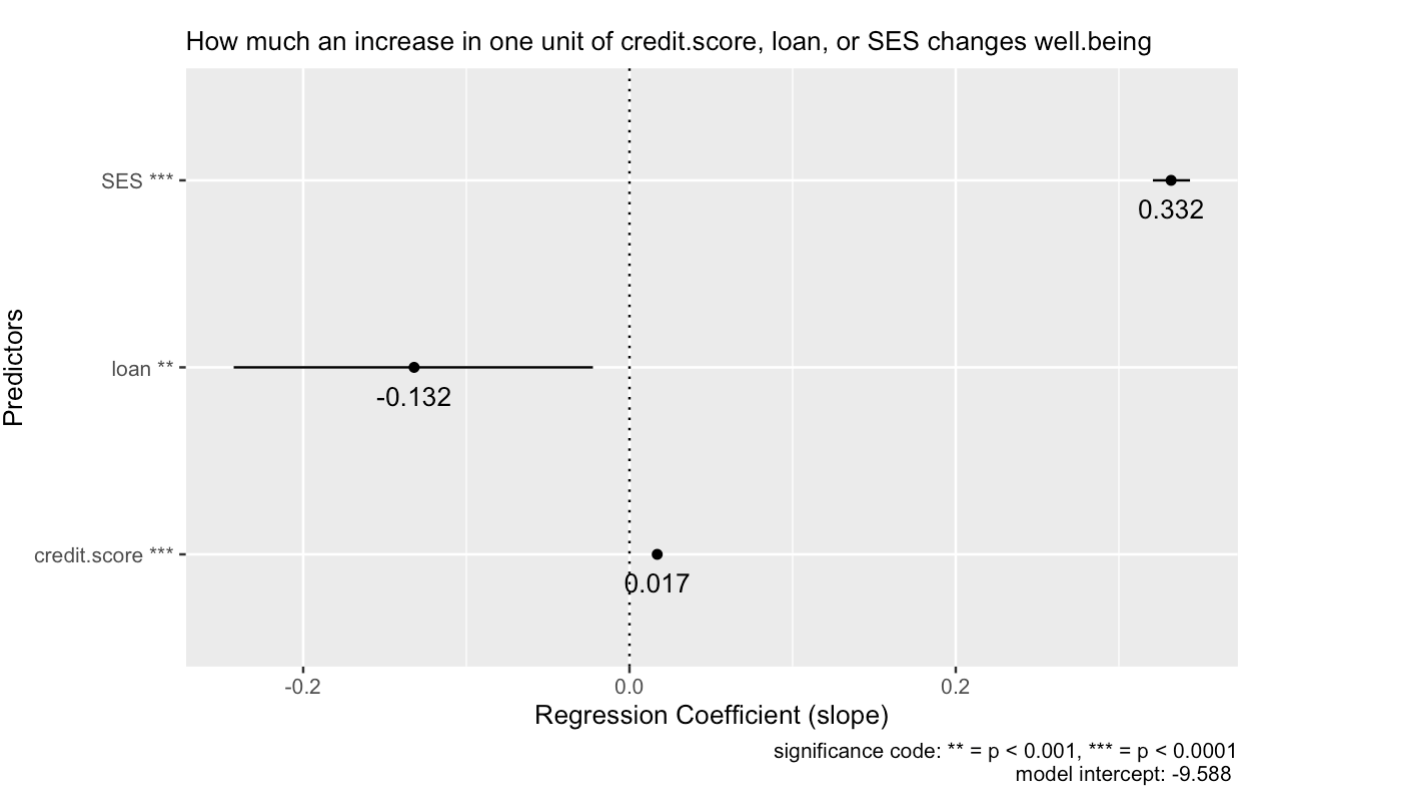
\includegraphics{figure-1.png}

Figure 1. Regression coefficient of credit score, loan, and SES to
describe the change in well-being per each unit increase.

Relative to other predictors, although still significant, loan has the
least significant effect towards well-being, \(F(1,4996)=7.456\),
\(p = .006\). This is expected since loan and credit.score are highly
correlated, \(R^2\) = .494, whilst credit score can explain well-being
better than loan, \(R^2\) = .494 and \(R^2\) = .354 respectively. Thus,
making the model shifts its attention more to credit score than loan
when it comes to predicting well-being.

As for the magnitude of change, holding credit.score and SES constant,
one unit increase on loan variable predicts a decrease of .132 unit of
well-being 95\% CI{[}(-.242) -- (-.022){]}. Such change is significant,
\(t(4996) = -2.359\), \(p < .001\).

\begin{center}\rule{0.5\linewidth}{\linethickness}\end{center}

\hypertarget{does-taking-payday-loan-makes-people-more-or-less-likely-to-experience-an-adverse-credit-event}{%
\section{Does taking payday loan makes people more or less likely to
experience an adverse credit
event?}\label{does-taking-payday-loan-makes-people-more-or-less-likely-to-experience-an-adverse-credit-event}}

\begin{quote}
Those taking payday loan are less likely to experience adverse credit
event. And Social Economic Status does not have a significant effect on
adverse credit event nor on the relationship loan has with adverse
credit event.
\end{quote}

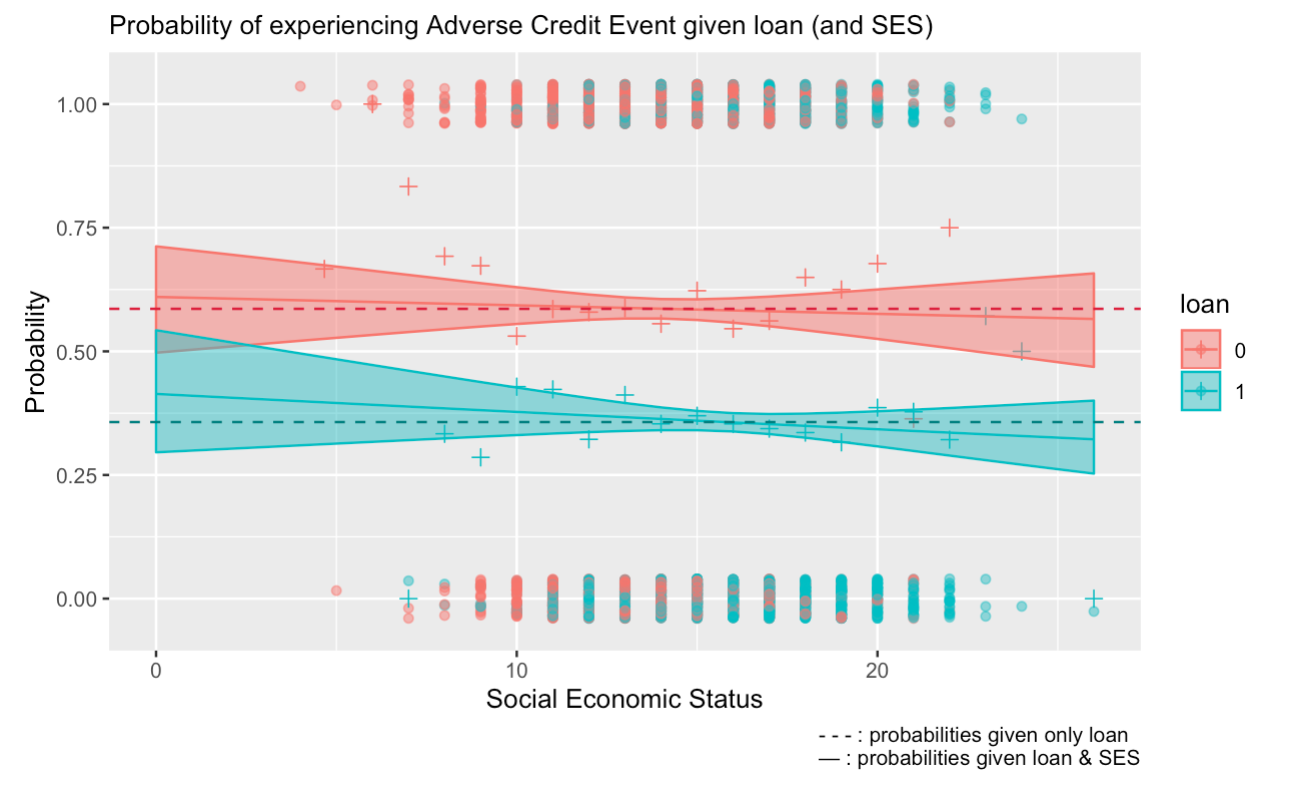
\includegraphics{figure-2.png} Figure 2. A comparison of probability
estimate on adverse credit event given loan (and SES)

Figure 2 describes the difference in probability of experiencing adverse
credit event (ACE) when receiving a loan and a comparison of how
insignificant SES affect the probabilities as SES increases. The dashed
line is the probability estimate for ACE given a loan or not (without
SES), the dots describes the individuals who either experienced ACE or
not, the +s are the proportion of ACE in each SES rank, while the line
and ribbon are the fit of a logistic regression model and its 95\% CI
given SES.

The effects of loan on ACE is significant, \(\chi^2(4998)\)=6644.6,
\(p\)\textless{}.0001. In contrast, SES has almost no effect on ACE,
\(\chi^2\)(4997)=6643.7, \(p\)=.339 nor on the relationship loan has
with ACE, \(\chi^2(4996)\)=6643.6, \(p\)=.339.

The probability of those taking payday loan to experience ACE, .357 95\%
CI{[}.339 -- .376{]}, is lower than those who do not, .586 95\%
CI{[}.566 -- .606{]}, about an absolute .229 change in probability.

\begin{center}\rule{0.5\linewidth}{\linethickness}\end{center}

\hypertarget{in-depth-analysis}{%
\section{In-depth Analysis}\label{in-depth-analysis}}

\begin{Shaded}
\begin{Highlighting}[]
\CommentTok{# --------- Exploratory Data Analysis}

\KeywordTok{summary}\NormalTok{(payday)}
\end{Highlighting}
\end{Shaded}

\begin{verbatim}
##   credit.score        SES          loan          well.being    adverse.credit.event
##  Min.   :400.0   Min.   : 4   Min.   :0.0000   Min.   :1.000   Min.   :0.0000      
##  1st Qu.:450.0   1st Qu.:13   1st Qu.:0.0000   1st Qu.:3.000   1st Qu.:0.0000      
##  Median :500.0   Median :15   Median :1.0000   Median :4.000   Median :0.0000      
##  Mean   :499.3   Mean   :15   Mean   :0.5178   Mean   :4.011   Mean   :0.4674      
##  3rd Qu.:550.0   3rd Qu.:17   3rd Qu.:1.0000   3rd Qu.:5.000   3rd Qu.:1.0000      
##  Max.   :600.0   Max.   :26   Max.   :1.0000   Max.   :7.000   Max.   :1.0000
\end{verbatim}

\begin{Shaded}
\begin{Highlighting}[]
\KeywordTok{plot_histogram}\NormalTok{(payday)}
\end{Highlighting}
\end{Shaded}

\includegraphics{1992799_files/figure-latex/question-1: EDA-1.pdf}

\begin{Shaded}
\begin{Highlighting}[]
\KeywordTok{pairs}\NormalTok{(payday, }\DataTypeTok{panel=}\NormalTok{panel.smooth)}
\end{Highlighting}
\end{Shaded}

\includegraphics{1992799_files/figure-latex/question-1: EDA-2.pdf}

\begin{Shaded}
\begin{Highlighting}[]
\KeywordTok{plot_correlation}\NormalTok{(payday)}
\end{Highlighting}
\end{Shaded}

\includegraphics{1992799_files/figure-latex/question-1: EDA-3.pdf}

\begin{Shaded}
\begin{Highlighting}[]
\KeywordTok{grid.arrange}\NormalTok{(}
    \KeywordTok{ggplot}\NormalTok{(payday, }\KeywordTok{aes}\NormalTok{(}\DataTypeTok{y=}\NormalTok{well.being, }\DataTypeTok{x=}\NormalTok{credit.score,}\DataTypeTok{colour=}\KeywordTok{as.factor}\NormalTok{(payday}\OperatorTok{$}\NormalTok{loan))) }\OperatorTok{+}\StringTok{ }\KeywordTok{geom_point}\NormalTok{(}\DataTypeTok{mapping =} \KeywordTok{aes}\NormalTok{(}\DataTypeTok{colour=}\KeywordTok{as.factor}\NormalTok{(payday}\OperatorTok{$}\NormalTok{loan))) }\OperatorTok{+}\StringTok{ }\KeywordTok{scale_y_continuous}\NormalTok{(}\DataTypeTok{breaks =} \DecValTok{1}\OperatorTok{:}\DecValTok{7}\NormalTok{) }\OperatorTok{+}\KeywordTok{labs}\NormalTok{(}\DataTypeTok{x=}\StringTok{"Credit score"}\NormalTok{, }\DataTypeTok{y=}\StringTok{"Well-being"}\NormalTok{,}\DataTypeTok{title=}\StringTok{"Relationship between credit.score and well.being by loan"}\NormalTok{,}\DataTypeTok{col=}\StringTok{"Loan"}\NormalTok{) }\OperatorTok{+}\StringTok{ }\KeywordTok{geom_smooth}\NormalTok{(}\DataTypeTok{method=}\NormalTok{lm),}
    
    \KeywordTok{ggplot}\NormalTok{(payday, }\KeywordTok{aes}\NormalTok{(}\DataTypeTok{y=}\NormalTok{well.being, }\DataTypeTok{x=}\NormalTok{SES,}\DataTypeTok{colour=}\KeywordTok{as.factor}\NormalTok{(payday}\OperatorTok{$}\NormalTok{loan))) }\OperatorTok{+}\StringTok{ }\KeywordTok{geom_jitter}\NormalTok{() }\OperatorTok{+}\KeywordTok{scale_y_continuous}\NormalTok{(}\DataTypeTok{breaks =} \DecValTok{1}\OperatorTok{:}\DecValTok{7}\NormalTok{)}\OperatorTok{+}\StringTok{ }\KeywordTok{labs}\NormalTok{(}\DataTypeTok{x=}\StringTok{"Social Economic Status"}\NormalTok{, }\DataTypeTok{y=}\StringTok{"Well-being"}\NormalTok{,}\DataTypeTok{title=}\StringTok{"Relationship between SES and well.being by loan"}\NormalTok{,}\DataTypeTok{col=}\StringTok{"Loan"}\NormalTok{) }\OperatorTok{+}\KeywordTok{geom_smooth}\NormalTok{(}\DataTypeTok{method=}\NormalTok{lm))}
\end{Highlighting}
\end{Shaded}

\includegraphics{1992799_files/figure-latex/question-1: EDA-4.pdf}

\begin{Shaded}
\begin{Highlighting}[]
\CommentTok{#  --------- Compute R^2 among variables to understand the multicoliniarity.}
\KeywordTok{round}\NormalTok{((}\KeywordTok{cor}\NormalTok{(payday))}\OperatorTok{^}\DecValTok{2}\NormalTok{, }\DataTypeTok{digits =} \DecValTok{3}\NormalTok{)}
\end{Highlighting}
\end{Shaded}

\begin{verbatim}
##                      credit.score   SES  loan well.being adverse.credit.event
## credit.score                1.000 0.148 0.743      0.494                0.071
## SES                         0.148 1.000 0.108      0.467                0.008
## loan                        0.743 0.108 1.000      0.354                0.053
## well.being                  0.494 0.467 0.354      1.000                0.030
## adverse.credit.event        0.071 0.008 0.053      0.030                1.000
\end{verbatim}

\texttt{loan} and \texttt{credit.score} has relatively high correlation
with each other (\(R^2 = .743\)), . However, \texttt{credit.score}
(\(R^2 = .494\)) can explain well.being better than loan
(\(R^2 = .354\)). Therefore, it is within expectation that
\texttt{credit.score} might be a more significant independant variable
than loan in a multiple regression for well.being.

\begin{Shaded}
\begin{Highlighting}[]
\CommentTok{# --------- Linear regression on bivariate}
\NormalTok{LM_loan <-}\StringTok{ }\KeywordTok{lm}\NormalTok{(well.being}\OperatorTok{~}\StringTok{ }\NormalTok{loan, }\DataTypeTok{data=}\NormalTok{payday)}
\NormalTok{LM_credit.score <-}\StringTok{ }\KeywordTok{lm}\NormalTok{(well.being}\OperatorTok{~}\StringTok{ }\NormalTok{credit.score, }\DataTypeTok{data=}\NormalTok{payday) }
\NormalTok{LM_ses <-}\StringTok{ }\KeywordTok{lm}\NormalTok{(well.being}\OperatorTok{~}\StringTok{ }\NormalTok{SES, }\DataTypeTok{data=}\NormalTok{payday) }

\CommentTok{# --------- Multiple regression models for well.being}
\NormalTok{LM_credit.loan <-}\StringTok{ }\KeywordTok{lm}\NormalTok{(well.being}\OperatorTok{~}\StringTok{ }\NormalTok{credit.score }\OperatorTok{+}\StringTok{ }\NormalTok{loan, }\DataTypeTok{data=}\NormalTok{payday) }\CommentTok{# model1, without SES }
\NormalTok{LM_credit.loan.ses <-}\StringTok{ }\KeywordTok{lm}\NormalTok{(well.being }\OperatorTok{~}\StringTok{ }\NormalTok{credit.score }\OperatorTok{+}\StringTok{ }\NormalTok{loan }\OperatorTok{+}\StringTok{ }\NormalTok{SES , }\DataTypeTok{data=}\NormalTok{payday)  }\CommentTok{# model2, including SES}
\end{Highlighting}
\end{Shaded}

\texttt{LM\_credit.loan} has loan and credit.score as independent
variables for well.being. While, \texttt{LM\_credit.loan.ses} in
addition to what \texttt{LM\_credit.loan} has, SES is added.

\begin{Shaded}
\begin{Highlighting}[]
\CommentTok{# --------- NHST whether the variables are significant in a bivariate setup}
\KeywordTok{anova}\NormalTok{(LM_loan) }
\end{Highlighting}
\end{Shaded}

\begin{verbatim}
## Analysis of Variance Table
## 
## Response: well.being
##             Df  Sum Sq Mean Sq F value    Pr(>F)    
## loan         1  5852.6  5852.6  2738.6 < 2.2e-16 ***
## Residuals 4998 10680.9     2.1                      
## ---
## Signif. codes:  0 '***' 0.001 '**' 0.01 '*' 0.05 '.' 0.1 ' ' 1
\end{verbatim}

\begin{Shaded}
\begin{Highlighting}[]
\KeywordTok{anova}\NormalTok{(LM_credit.score)}
\end{Highlighting}
\end{Shaded}

\begin{verbatim}
## Analysis of Variance Table
## 
## Response: well.being
##                Df Sum Sq Mean Sq F value    Pr(>F)    
## credit.score    1 8163.1  8163.1  4874.3 < 2.2e-16 ***
## Residuals    4998 8370.3     1.7                      
## ---
## Signif. codes:  0 '***' 0.001 '**' 0.01 '*' 0.05 '.' 0.1 ' ' 1
\end{verbatim}

\begin{Shaded}
\begin{Highlighting}[]
\KeywordTok{anova}\NormalTok{(LM_ses)}
\end{Highlighting}
\end{Shaded}

\begin{verbatim}
## Analysis of Variance Table
## 
## Response: well.being
##             Df Sum Sq Mean Sq F value    Pr(>F)    
## SES          1 7722.4  7722.4  4380.5 < 2.2e-16 ***
## Residuals 4998 8811.0     1.8                      
## ---
## Signif. codes:  0 '***' 0.001 '**' 0.01 '*' 0.05 '.' 0.1 ' ' 1
\end{verbatim}

\begin{Shaded}
\begin{Highlighting}[]
\CommentTok{# --------- NHST whether the variance differ between multiple regression model with and without SES}
\CommentTok{#H0: LM_credit.loan == LM_credit.loan.ses ; HA: LM_credit.loan != LM_credit.loan.ses }
\KeywordTok{anova}\NormalTok{(LM_credit.loan, LM_credit.loan.ses) }
\end{Highlighting}
\end{Shaded}

\begin{verbatim}
## Analysis of Variance Table
## 
## Model 1: well.being ~ credit.score + loan
## Model 2: well.being ~ credit.score + loan + SES
##   Res.Df    RSS Df Sum of Sq      F    Pr(>F)    
## 1   4997 8362.8                                  
## 2   4996 5053.0  1    3309.8 3272.5 < 2.2e-16 ***
## ---
## Signif. codes:  0 '***' 0.001 '**' 0.01 '*' 0.05 '.' 0.1 ' ' 1
\end{verbatim}

\begin{Shaded}
\begin{Highlighting}[]
\CommentTok{# --------- NHST the significance of the variables}
\CommentTok{# For each variable... H0: model with variable == model without variable ; HA: model with variable != model without variable}
\KeywordTok{anova}\NormalTok{(LM_credit.loan.ses) }
\end{Highlighting}
\end{Shaded}

\begin{verbatim}
## Analysis of Variance Table
## 
## Response: well.being
##                Df Sum Sq Mean Sq   F value    Pr(>F)    
## credit.score    1 8163.1  8163.1 8071.0331 < 2.2e-16 ***
## loan            1    7.5     7.5    7.4561  0.006344 ** 
## SES             1 3309.8  3309.8 3272.4871 < 2.2e-16 ***
## Residuals    4996 5053.0     1.0                        
## ---
## Signif. codes:  0 '***' 0.001 '**' 0.01 '*' 0.05 '.' 0.1 ' ' 1
\end{verbatim}

All bivariate LMs has significant effect on \texttt{well.being}, but
when put together, the significance of loan shifts to
\texttt{credit.score}. This comes back again to the fact that
\texttt{credit.score} and \texttt{loan} are highly correlated. But
\texttt{credit.score} still have the upperhand when it comes to
predicting \texttt{well.being}.

The \texttt{LM\_credit.loan.ses} fits significantly better, F=3272.5 and
p \textless{} .0001, with an increase of 0.2 in \(R^2\) and a decrease
in 3309 of RSS compared to \texttt{LM\_credit.loan}. We can say that
adding \texttt{SES} explains an additional 20\% of the variance in well
being and it is statistically significant.

All independent variables in \texttt{LM\_credit.loan.ses} are
significant, but compared to \texttt{credit.score} and
\texttt{credit.score}, \texttt{loan} is the least significant, p=.006.

\begin{Shaded}
\begin{Highlighting}[]
\CommentTok{# --------- the equation for wellbeing}
\KeywordTok{summary}\NormalTok{(LM_credit.loan.ses)}
\end{Highlighting}
\end{Shaded}

\begin{verbatim}
## 
## Call:
## lm(formula = well.being ~ credit.score + loan + SES, data = payday)
## 
## Residuals:
##     Min      1Q  Median      3Q     Max 
## -3.8283 -0.6951  0.0084  0.6656  3.7784 
## 
## Coefficients:
##                Estimate Std. Error t value Pr(>|t|)    
## (Intercept)  -9.5881336  0.2233281 -42.933   <2e-16 ***
## credit.score  0.0173921  0.0005017  34.667   <2e-16 ***
## loan         -0.1324966  0.0561764  -2.359   0.0184 *  
## SES           0.3322207  0.0058075  57.206   <2e-16 ***
## ---
## Signif. codes:  0 '***' 0.001 '**' 0.01 '*' 0.05 '.' 0.1 ' ' 1
## 
## Residual standard error: 1.006 on 4996 degrees of freedom
## Multiple R-squared:  0.6944, Adjusted R-squared:  0.6942 
## F-statistic:  3784 on 3 and 4996 DF,  p-value: < 2.2e-16
\end{verbatim}

\begin{Shaded}
\begin{Highlighting}[]
\KeywordTok{cbind}\NormalTok{(}\KeywordTok{coef}\NormalTok{(LM_credit.loan.ses), }\KeywordTok{confint}\NormalTok{(LM_credit.loan.ses)) }\CommentTok{#Confidence interval of the estimate}
\end{Highlighting}
\end{Shaded}

\begin{verbatim}
##                                 2.5 %      97.5 %
## (Intercept)  -9.58813364 -10.02595471 -9.15031256
## credit.score  0.01739205   0.01640852  0.01837558
## loan         -0.13249660  -0.24262709 -0.02236611
## SES           0.33222068   0.32083547  0.34360589
\end{verbatim}

\texttt{well.being} can be explained through the following equation:
\(\widehat{well.being} = -9.588 + 0.017 \times credit.score - 0.132 \times loan + 0.332 \times SES\)

As for the magnitude of change, holding \texttt{credit.score} and
\texttt{SES} constant, one unit increase on loan variable predicts a
decrease of .132 units on \texttt{well.being} 95\% CI{[}(-.242) --
(-.022){]}. Such change is significant, \(t(4996) = -2.359\),
\(p < .001\).

The negative coefficient of \texttt{loan} can be explained by the
multiple colinearity with \texttt{credit.score}, the binary input, and
the constraint of 7 scales of \texttt{well.being}. Simply put,
\texttt{loan} balances \texttt{credit.score}'s impact by going to the
opposite direction when \texttt{loan} == 1.

\begin{Shaded}
\begin{Highlighting}[]
\CommentTok{# --------- plot prep}
\NormalTok{df_coeff <-}\StringTok{ }\KeywordTok{as.data.frame}\NormalTok{(}\KeywordTok{cbind}\NormalTok{(}\KeywordTok{coef}\NormalTok{(LM_credit.loan.ses), }\KeywordTok{confint}\NormalTok{(LM_credit.loan.ses)))}
\NormalTok{df_coeff <-}\StringTok{ }\KeywordTok{mutate}\NormalTok{(df_coeff, }\DataTypeTok{id =} \KeywordTok{rownames}\NormalTok{(df_coeff))}
\NormalTok{df_coeff <-}\StringTok{ }\KeywordTok{anti_join}\NormalTok{(df_coeff, }\KeywordTok{subset}\NormalTok{(df_coeff, id}\OperatorTok{==}\StringTok{'(Intercept)'}\NormalTok{))}
\end{Highlighting}
\end{Shaded}

\begin{verbatim}
## Joining, by = c("V1", "2.5 %", "97.5 %", "id")
\end{verbatim}

\begin{Shaded}
\begin{Highlighting}[]
\NormalTok{df_coeff <-}\StringTok{ }\NormalTok{df_coeff }\OperatorTok
\StringTok{  }\KeywordTok{mutate}\NormalTok{(}\DataTypeTok{V1 =} \KeywordTok{round}\NormalTok{(V1,}\DataTypeTok{digits =} \DecValTok{3}\NormalTok{))}

\NormalTok{df_coeff}\OperatorTok{$}\NormalTok{id[df_coeff}\OperatorTok{$}\NormalTok{id }\OperatorTok{==}\StringTok{ "credit.score"}\NormalTok{] <-}\StringTok{ "credit.score ***"}
\NormalTok{df_coeff}\OperatorTok{$}\NormalTok{id[df_coeff}\OperatorTok{$}\NormalTok{id }\OperatorTok{==}\StringTok{ "loan"}\NormalTok{] <-}\StringTok{ "loan **"}
\NormalTok{df_coeff}\OperatorTok{$}\NormalTok{id[df_coeff}\OperatorTok{$}\NormalTok{id }\OperatorTok{==}\StringTok{ "SES"}\NormalTok{] <-}\StringTok{ "SES ***"}

\CommentTok{# --------- plotting}
\KeywordTok{ggplot}\NormalTok{(df_coeff , }\KeywordTok{aes}\NormalTok{(}\DataTypeTok{y=}\KeywordTok{as.factor}\NormalTok{(id), }\DataTypeTok{x=}\NormalTok{V1)) }\OperatorTok{+}\StringTok{ }
\StringTok{  }\KeywordTok{geom_point}\NormalTok{() }\OperatorTok{+}\StringTok{ }\KeywordTok{geom_text}\NormalTok{(}\KeywordTok{aes}\NormalTok{(}\DataTypeTok{label=}\NormalTok{V1),}\DataTypeTok{hjust=}\FloatTok{0.5}\NormalTok{, }\DataTypeTok{vjust=}\DecValTok{2}\NormalTok{) }\OperatorTok{+}
\StringTok{  }\KeywordTok{labs}\NormalTok{(}\DataTypeTok{x=}\StringTok{"Regression Coefficient (slope)"}\NormalTok{, }\DataTypeTok{y=}\StringTok{"Predictors"}\NormalTok{,}\DataTypeTok{subtitle=}\StringTok{"How much an increase in one unit of credit.score, loan, or SES changes well.being"}\NormalTok{, }\DataTypeTok{caption =} \StringTok{"significance code: ** = p < 0.001, *** = p < 0.0001}\CharTok{\textbackslash{}n}\StringTok{ model intercept: -9.588 "}\NormalTok{ ) }\OperatorTok{+}\StringTok{ }
\StringTok{  }\KeywordTok{geom_segment}\NormalTok{(}\KeywordTok{aes}\NormalTok{(}\DataTypeTok{x=}\StringTok{`}\DataTypeTok{2.5 %}\StringTok{`}\NormalTok{,}\DataTypeTok{xend=}\StringTok{`}\DataTypeTok{97.5 %}\StringTok{`}\NormalTok{,}\DataTypeTok{y=}\KeywordTok{as.factor}\NormalTok{(id),}\DataTypeTok{yend=}\KeywordTok{as.factor}\NormalTok{(id) )) }\OperatorTok{+}\StringTok{ }
\StringTok{  }\KeywordTok{geom_vline}\NormalTok{(}\DataTypeTok{xintercept =} \DecValTok{0}\NormalTok{, }\DataTypeTok{linetype=}\StringTok{'dotted'}\NormalTok{)}
\end{Highlighting}
\end{Shaded}

\includegraphics{1992799_files/figure-latex/question-1: mainplot-1.pdf}

\begin{center}\rule{0.5\linewidth}{\linethickness}\end{center}

\begin{Shaded}
\begin{Highlighting}[]
\CommentTok{# --------- Exploratory Data Analysis}
\NormalTok{mu <-}\StringTok{ }\NormalTok{payday }\OperatorTok
\StringTok{    }\KeywordTok{group_by}\NormalTok{(adverse.credit.event) }\OperatorTok
\StringTok{    }\KeywordTok{summarise}\NormalTok{(}\DataTypeTok{mean=}\KeywordTok{mean}\NormalTok{(credit.score))}

\KeywordTok{ggplot}\NormalTok{(payday, }\KeywordTok{aes}\NormalTok{(}\DataTypeTok{x=}\NormalTok{credit.score, }\DataTypeTok{color=}\KeywordTok{as.factor}\NormalTok{(adverse.credit.event), }\DataTypeTok{fill=}\KeywordTok{as.factor}\NormalTok{(adverse.credit.event))) }\OperatorTok{+}
\StringTok{  }\KeywordTok{geom_histogram}\NormalTok{(}\DataTypeTok{alpha =}\FloatTok{0.5}\NormalTok{, }\DataTypeTok{position=}\StringTok{"dodge"}\NormalTok{, }\DataTypeTok{bins =} \DecValTok{50}\NormalTok{)}\OperatorTok{+}
\StringTok{  }\KeywordTok{geom_density}\NormalTok{(}\DataTypeTok{alpha=}\FloatTok{0.6}\NormalTok{)}\OperatorTok{+}
\StringTok{  }\KeywordTok{geom_vline}\NormalTok{(}\DataTypeTok{data=}\NormalTok{mu, }\KeywordTok{aes}\NormalTok{(}\DataTypeTok{xintercept=}\NormalTok{mean, }\DataTypeTok{color=}\KeywordTok{as.factor}\NormalTok{(adverse.credit.event)),}\DataTypeTok{linetype=}\StringTok{"dashed"}\NormalTok{)}\OperatorTok{+}
\StringTok{  }\KeywordTok{geom_vline}\NormalTok{(}\DataTypeTok{xintercept =} \DecValTok{500}\NormalTok{, }\DataTypeTok{colour=}\StringTok{"#990000"}\NormalTok{, }\DataTypeTok{linetype=}\StringTok{"longdash"}\NormalTok{)}\OperatorTok{+}
\StringTok{  }\KeywordTok{scale_color_manual}\NormalTok{(}\DataTypeTok{values=}\KeywordTok{c}\NormalTok{(}\StringTok{"#999999"}\NormalTok{, }\StringTok{"#E69F00"}\NormalTok{, }\StringTok{"#56B4E9"}\NormalTok{))}\OperatorTok{+}
\StringTok{  }\KeywordTok{scale_fill_manual}\NormalTok{(}\DataTypeTok{values=}\KeywordTok{c}\NormalTok{(}\StringTok{"#999999"}\NormalTok{, }\StringTok{"#E69F00"}\NormalTok{, }\StringTok{"#56B4E9"}\NormalTok{))}\OperatorTok{+}
\StringTok{  }\KeywordTok{theme}\NormalTok{(}\DataTypeTok{legend.position=}\StringTok{"top"}\NormalTok{) }
\end{Highlighting}
\end{Shaded}

\includegraphics{1992799_files/figure-latex/question-2: EDA-1.pdf}

\begin{Shaded}
\begin{Highlighting}[]
\CommentTok{# --------- Build logistic regression model }
\NormalTok{adverse.by.loan.ses <-}\StringTok{ }\KeywordTok{glm}\NormalTok{(adverse.credit.event}\OperatorTok{~}\NormalTok{loan}\OperatorTok{*}\NormalTok{SES , }\DataTypeTok{family=}\NormalTok{binomial, }\DataTypeTok{data=}\NormalTok{payday)}
\NormalTok{adverse.by.loan <-}\StringTok{ }\KeywordTok{glm}\NormalTok{(adverse.credit.event}\OperatorTok{~}\NormalTok{loan, }\DataTypeTok{family=}\NormalTok{binomial, }\DataTypeTok{data=}\NormalTok{payday)}

\KeywordTok{summary}\NormalTok{(adverse.by.loan.ses)}
\end{Highlighting}
\end{Shaded}

\begin{verbatim}
## 
## Call:
## glm(formula = adverse.credit.event ~ loan * SES, family = binomial, 
##     data = payday)
## 
## Deviance Residuals: 
##     Min       1Q   Median       3Q      Max  
## -1.3567  -0.9561  -0.9214   1.0392   1.4914  
## 
## Coefficients:
##              Estimate Std. Error z value Pr(>|z|)  
## (Intercept)  0.447556   0.234026   1.912   0.0558 .
## loan        -0.795326   0.353494  -2.250   0.0245 *
## SES         -0.007080   0.016331  -0.434   0.6646  
## loan:SES    -0.008152   0.023251  -0.351   0.7259  
## ---
## Signif. codes:  0 '***' 0.001 '**' 0.01 '*' 0.05 '.' 0.1 ' ' 1
## 
## (Dispersion parameter for binomial family taken to be 1)
## 
##     Null deviance: 6910.2  on 4999  degrees of freedom
## Residual deviance: 6643.6  on 4996  degrees of freedom
## AIC: 6651.6
## 
## Number of Fisher Scoring iterations: 4
\end{verbatim}

\begin{Shaded}
\begin{Highlighting}[]
\KeywordTok{summary}\NormalTok{(adverse.by.loan)}
\end{Highlighting}
\end{Shaded}

\begin{verbatim}
## 
## Call:
## glm(formula = adverse.credit.event ~ loan, family = binomial, 
##     data = payday)
## 
## Deviance Residuals: 
##     Min       1Q   Median       3Q      Max  
## -1.3282  -0.9396  -0.9396   1.0338   1.4355  
## 
## Coefficients:
##             Estimate Std. Error z value Pr(>|z|)    
## (Intercept)  0.34772    0.04135   8.409   <2e-16 ***
## loan        -0.93659    0.05825 -16.080   <2e-16 ***
## ---
## Signif. codes:  0 '***' 0.001 '**' 0.01 '*' 0.05 '.' 0.1 ' ' 1
## 
## (Dispersion parameter for binomial family taken to be 1)
## 
##     Null deviance: 6910.2  on 4999  degrees of freedom
## Residual deviance: 6644.6  on 4998  degrees of freedom
## AIC: 6648.6
## 
## Number of Fisher Scoring iterations: 4
\end{verbatim}

\begin{Shaded}
\begin{Highlighting}[]
\CommentTok{# --------- Get the probability of adverse credit event by loan and its estimation}
\NormalTok{adverse.by.loan.emm <-}\StringTok{ }\KeywordTok{emmeans}\NormalTok{(adverse.by.loan, }\OperatorTok{~}\NormalTok{loan, }\DataTypeTok{type=}\StringTok{"response"}\NormalTok{)}
\KeywordTok{confint}\NormalTok{(adverse.by.loan.emm)}
\end{Highlighting}
\end{Shaded}

\begin{verbatim}
##  loan  prob      SE  df asymp.LCL asymp.UCL
##     0 0.586 0.01003 Inf     0.566     0.606
##     1 0.357 0.00942 Inf     0.339     0.376
## 
## Confidence level used: 0.95 
## Intervals are back-transformed from the logit scale
\end{verbatim}

\begin{Shaded}
\begin{Highlighting}[]
\CommentTok{# --------- Plot the probabilities}
\KeywordTok{ggplot}\NormalTok{(}\KeywordTok{summary}\NormalTok{(adverse.by.loan.emm), }\KeywordTok{aes}\NormalTok{(}\DataTypeTok{x=}\KeywordTok{as.factor}\NormalTok{(loan), }\DataTypeTok{y=}\NormalTok{prob, }\DataTypeTok{ymin=}\NormalTok{asymp.LCL, }\DataTypeTok{ymax=}\NormalTok{asymp.UCL)) }\OperatorTok{+}\StringTok{ }\KeywordTok{geom_point}\NormalTok{() }\OperatorTok{+}\StringTok{ }\KeywordTok{geom_linerange}\NormalTok{() }\OperatorTok{+}\StringTok{ }\KeywordTok{labs}\NormalTok{(}\DataTypeTok{x=}\StringTok{"Loan"}\NormalTok{, }\DataTypeTok{y=}\StringTok{"Proportion of adverse credit event"}\NormalTok{)  }\OperatorTok{+}
\StringTok{  }\KeywordTok{geom_hline}\NormalTok{(}\DataTypeTok{yintercept =} \FloatTok{0.586}\NormalTok{, }\DataTypeTok{lty=}\DecValTok{2}\NormalTok{) }\OperatorTok{+}
\StringTok{  }\KeywordTok{geom_hline}\NormalTok{(}\DataTypeTok{yintercept =} \FloatTok{0.357}\NormalTok{, }\DataTypeTok{lty=}\DecValTok{2}\NormalTok{)}
\end{Highlighting}
\end{Shaded}

\includegraphics{1992799_files/figure-latex/question-2: model fitting, NHST, and Estimation-1.pdf}

\begin{Shaded}
\begin{Highlighting}[]
\CommentTok{# --------- Prove that SES is insignificant for explaining adverse.credit.event}
\KeywordTok{anova}\NormalTok{(adverse.by.loan.ses, }\DataTypeTok{test=}\StringTok{"Chisq"}\NormalTok{)}
\end{Highlighting}
\end{Shaded}

\begin{verbatim}
## Analysis of Deviance Table
## 
## Model: binomial, link: logit
## 
## Response: adverse.credit.event
## 
## Terms added sequentially (first to last)
## 
## 
##          Df Deviance Resid. Df Resid. Dev Pr(>Chi)    
## NULL                      4999     6910.2             
## loan      1  265.597      4998     6644.6   <2e-16 ***
## SES       1    0.913      4997     6643.7   0.3394    
## loan:SES  1    0.123      4996     6643.6   0.7259    
## ---
## Signif. codes:  0 '***' 0.001 '**' 0.01 '*' 0.05 '.' 0.1 ' ' 1
\end{verbatim}

A change of probability of ACE between receiving a loan and not
receiving one is about an absolute 22.9\%. Additionally, SES has almost
no effect on ACE, \(\chi^2\)(4997)=6643.7, \(p\)=.339 nor on the
relationship loan has with ACE, \(\chi^2(4996)\)=6643.6, \(p\)=.339.

\begin{Shaded}
\begin{Highlighting}[]
\CommentTok{# --------- Plot Prep}
\NormalTok{adverse.by.loan.ses.emm <-}\StringTok{ }\KeywordTok{emmeans}\NormalTok{(adverse.by.loan.ses, }\OperatorTok{~}\NormalTok{loan}\OperatorTok{*}\NormalTok{SES, }\DataTypeTok{at=}\KeywordTok{list}\NormalTok{(}\DataTypeTok{SES=}\KeywordTok{seq}\NormalTok{(}\DecValTok{0}\NormalTok{,}\DecValTok{26}\NormalTok{,}\DecValTok{1}\NormalTok{)), }\DataTypeTok{type=}\StringTok{"response"}\NormalTok{)}
\NormalTok{ses.unique<-}\StringTok{ }\KeywordTok{unique}\NormalTok{(payday}\OperatorTok{$}\NormalTok{SES)}
\NormalTok{payday_t <-}\StringTok{ }\NormalTok{payday }\OperatorTok\StringTok{ }
\StringTok{  }\KeywordTok{mutate}\NormalTok{(}\DataTypeTok{SES.deciles=}\KeywordTok{cut}\NormalTok{(SES, }\DataTypeTok{breaks=}\NormalTok{ses.unique, }\DataTypeTok{include.lowest=}\OtherTok{TRUE}\NormalTok{))}

\NormalTok{payday_t.loan.ses <-}\StringTok{ }\NormalTok{payday_t }\OperatorTok\StringTok{ }
\StringTok{  }\KeywordTok{group_by}\NormalTok{(SES.deciles,loan) }\OperatorTok\StringTok{ }
\StringTok{  }\KeywordTok{summarise}\NormalTok{(}\DataTypeTok{Proportion.adverse=}\KeywordTok{mean}\NormalTok{(adverse.credit.event), }\DataTypeTok{decile.mean.ses=}\KeywordTok{mean}\NormalTok{(SES))}

\NormalTok{payday_t}\OperatorTok{$}\NormalTok{loan <-}\StringTok{ }\KeywordTok{as.factor}\NormalTok{(payday_t}\OperatorTok{$}\NormalTok{loan)}
\NormalTok{payday_t.loan.ses}\OperatorTok{$}\NormalTok{loan <-}\StringTok{ }\KeywordTok{as.factor}\NormalTok{(payday_t.loan.ses}\OperatorTok{$}\NormalTok{loan)}


\NormalTok{sum_adverse.by.loan.ses.emm <-}\StringTok{ }\KeywordTok{as.data.frame}\NormalTok{(}\KeywordTok{summary}\NormalTok{(adverse.by.loan.ses.emm))}
\NormalTok{sum_adverse.by.loan.ses.emm}\OperatorTok{$}\NormalTok{loan <-}\StringTok{ }\KeywordTok{as.factor}\NormalTok{(sum_adverse.by.loan.ses.emm}\OperatorTok{$}\NormalTok{loan)}

\CommentTok{# --------- Plotting mainplot}
\KeywordTok{ggplot}\NormalTok{(sum_adverse.by.loan.ses.emm, }\KeywordTok{aes}\NormalTok{(}\DataTypeTok{x=}\NormalTok{SES, }\DataTypeTok{col=}\NormalTok{loan, }\DataTypeTok{fill=}\NormalTok{loan,}\DataTypeTok{y=}\NormalTok{prob, }\DataTypeTok{ymin=}\NormalTok{asymp.LCL, }\DataTypeTok{ymax=}\NormalTok{asymp.UCL)) }\OperatorTok{+}\StringTok{ }
\StringTok{    }\KeywordTok{geom_jitter}\NormalTok{(}\DataTypeTok{data=}\NormalTok{payday_t, }\DataTypeTok{mapping=}\KeywordTok{aes}\NormalTok{(}\DataTypeTok{y=}\NormalTok{adverse.credit.event, }\DataTypeTok{x=}\NormalTok{SES, }\DataTypeTok{col=}\NormalTok{loan,}\DataTypeTok{ymin=}\OtherTok{NULL}\NormalTok{, }\DataTypeTok{ymax=}\OtherTok{NULL}\NormalTok{), }\DataTypeTok{height=}\FloatTok{0.04}\NormalTok{, }\DataTypeTok{width=}\DecValTok{0}\NormalTok{, }\DataTypeTok{alpha=}\FloatTok{0.5}\NormalTok{) }\OperatorTok{+}\StringTok{ }
\StringTok{    }\KeywordTok{geom_point}\NormalTok{(}\DataTypeTok{data=}\NormalTok{payday_t.loan.ses, }\DataTypeTok{mapping=}\KeywordTok{aes}\NormalTok{(}\DataTypeTok{y=}\NormalTok{Proportion.adverse, }\DataTypeTok{x=}\NormalTok{decile.mean.ses, }\DataTypeTok{col=}\NormalTok{loan, }\DataTypeTok{ymin=}\OtherTok{NULL}\NormalTok{, }\DataTypeTok{ymax=}\OtherTok{NULL}\NormalTok{), }\DataTypeTok{size=}\DecValTok{2}\NormalTok{, }\DataTypeTok{shape=}\DecValTok{3}\NormalTok{) }\OperatorTok{+}
\StringTok{    }\KeywordTok{geom_ribbon}\NormalTok{(}\DataTypeTok{alpha =} \FloatTok{0.5}\NormalTok{) }\OperatorTok{+}\StringTok{ }
\StringTok{    }\KeywordTok{geom_line}\NormalTok{() }\OperatorTok{+}
\StringTok{    }\KeywordTok{labs}\NormalTok{(}\DataTypeTok{x=}\StringTok{"Social Economic Status"}\NormalTok{, }\DataTypeTok{y=}\StringTok{"Probability"}\NormalTok{, }\DataTypeTok{caption=}\StringTok{"- - - : probabilities given only loan  }\CharTok{\textbackslash{}n}\StringTok{  — : probabilities given loan & SES"}\NormalTok{, }\DataTypeTok{subtitle =} \StringTok{"Probability of experiencing Adverse Credit Event given loan (and SES)"}\NormalTok{ ) }\OperatorTok{+}\StringTok{ }
\StringTok{  }\KeywordTok{ylim}\NormalTok{(}\OperatorTok{-}\FloatTok{0.05}\NormalTok{,}\FloatTok{1.05}\NormalTok{) }\OperatorTok{+}
\StringTok{  }\KeywordTok{geom_hline}\NormalTok{(}\DataTypeTok{yintercept =} \FloatTok{0.586}\NormalTok{, }\DataTypeTok{lty=}\DecValTok{2}\NormalTok{, }\DataTypeTok{color=}\StringTok{'#DC143C'}\NormalTok{) }\OperatorTok{+}
\StringTok{  }\KeywordTok{geom_hline}\NormalTok{(}\DataTypeTok{yintercept =} \FloatTok{0.357}\NormalTok{, }\DataTypeTok{lty=}\DecValTok{2}\NormalTok{, }\DataTypeTok{color=}\StringTok{'#008080'}\NormalTok{)}
\end{Highlighting}
\end{Shaded}

\begin{verbatim}
## Warning in grid.Call(C_textBounds, as.graphicsAnnot(x$label), x$x, x$y, : conversion failure on '
## — : probabilities given loan & SES' in 'mbcsToSbcs': dot substituted for <e2>
\end{verbatim}

\begin{verbatim}
## Warning in grid.Call(C_textBounds, as.graphicsAnnot(x$label), x$x, x$y, : conversion failure on '
## — : probabilities given loan & SES' in 'mbcsToSbcs': dot substituted for <80>
\end{verbatim}

\begin{verbatim}
## Warning in grid.Call(C_textBounds, as.graphicsAnnot(x$label), x$x, x$y, : conversion failure on '
## — : probabilities given loan & SES' in 'mbcsToSbcs': dot substituted for <94>
\end{verbatim}

\begin{verbatim}
## Warning in grid.Call(C_textBounds, as.graphicsAnnot(x$label), x$x, x$y, : conversion failure on '
## — : probabilities given loan & SES' in 'mbcsToSbcs': dot substituted for <e2>
\end{verbatim}

\begin{verbatim}
## Warning in grid.Call(C_textBounds, as.graphicsAnnot(x$label), x$x, x$y, : conversion failure on '
## — : probabilities given loan & SES' in 'mbcsToSbcs': dot substituted for <80>
\end{verbatim}

\begin{verbatim}
## Warning in grid.Call(C_textBounds, as.graphicsAnnot(x$label), x$x, x$y, : conversion failure on '
## — : probabilities given loan & SES' in 'mbcsToSbcs': dot substituted for <94>
\end{verbatim}

\begin{verbatim}
## Warning in grid.Call(C_textBounds, as.graphicsAnnot(x$label), x$x, x$y, : conversion failure on '
## — : probabilities given loan & SES' in 'mbcsToSbcs': dot substituted for <e2>
\end{verbatim}

\begin{verbatim}
## Warning in grid.Call(C_textBounds, as.graphicsAnnot(x$label), x$x, x$y, : conversion failure on '
## — : probabilities given loan & SES' in 'mbcsToSbcs': dot substituted for <80>
\end{verbatim}

\begin{verbatim}
## Warning in grid.Call(C_textBounds, as.graphicsAnnot(x$label), x$x, x$y, : conversion failure on '
## — : probabilities given loan & SES' in 'mbcsToSbcs': dot substituted for <94>
\end{verbatim}

\begin{verbatim}
## Warning in grid.Call(C_textBounds, as.graphicsAnnot(x$label), x$x, x$y, : conversion failure on '
## — : probabilities given loan & SES' in 'mbcsToSbcs': dot substituted for <e2>
\end{verbatim}

\begin{verbatim}
## Warning in grid.Call(C_textBounds, as.graphicsAnnot(x$label), x$x, x$y, : conversion failure on '
## — : probabilities given loan & SES' in 'mbcsToSbcs': dot substituted for <80>
\end{verbatim}

\begin{verbatim}
## Warning in grid.Call(C_textBounds, as.graphicsAnnot(x$label), x$x, x$y, : conversion failure on '
## — : probabilities given loan & SES' in 'mbcsToSbcs': dot substituted for <94>
\end{verbatim}

\begin{verbatim}
## Warning in grid.Call(C_textBounds, as.graphicsAnnot(x$label), x$x, x$y, : conversion failure on '
## — : probabilities given loan & SES' in 'mbcsToSbcs': dot substituted for <e2>
\end{verbatim}

\begin{verbatim}
## Warning in grid.Call(C_textBounds, as.graphicsAnnot(x$label), x$x, x$y, : conversion failure on '
## — : probabilities given loan & SES' in 'mbcsToSbcs': dot substituted for <80>
\end{verbatim}

\begin{verbatim}
## Warning in grid.Call(C_textBounds, as.graphicsAnnot(x$label), x$x, x$y, : conversion failure on '
## — : probabilities given loan & SES' in 'mbcsToSbcs': dot substituted for <94>
\end{verbatim}

\begin{verbatim}
## Warning in grid.Call(C_textBounds, as.graphicsAnnot(x$label), x$x, x$y, : conversion failure on '
## — : probabilities given loan & SES' in 'mbcsToSbcs': dot substituted for <e2>
\end{verbatim}

\begin{verbatim}
## Warning in grid.Call(C_textBounds, as.graphicsAnnot(x$label), x$x, x$y, : conversion failure on '
## — : probabilities given loan & SES' in 'mbcsToSbcs': dot substituted for <80>
\end{verbatim}

\begin{verbatim}
## Warning in grid.Call(C_textBounds, as.graphicsAnnot(x$label), x$x, x$y, : conversion failure on '
## — : probabilities given loan & SES' in 'mbcsToSbcs': dot substituted for <94>
\end{verbatim}

\begin{verbatim}
## Warning in grid.Call(C_textBounds, as.graphicsAnnot(x$label), x$x, x$y, : conversion failure on '
## — : probabilities given loan & SES' in 'mbcsToSbcs': dot substituted for <e2>
\end{verbatim}

\begin{verbatim}
## Warning in grid.Call(C_textBounds, as.graphicsAnnot(x$label), x$x, x$y, : conversion failure on '
## — : probabilities given loan & SES' in 'mbcsToSbcs': dot substituted for <80>
\end{verbatim}

\begin{verbatim}
## Warning in grid.Call(C_textBounds, as.graphicsAnnot(x$label), x$x, x$y, : conversion failure on '
## — : probabilities given loan & SES' in 'mbcsToSbcs': dot substituted for <94>
\end{verbatim}

\begin{verbatim}
## Warning in grid.Call.graphics(C_text, as.graphicsAnnot(x$label), x$x, x$y, : conversion failure on '
## — : probabilities given loan & SES' in 'mbcsToSbcs': dot substituted for <e2>
\end{verbatim}

\begin{verbatim}
## Warning in grid.Call.graphics(C_text, as.graphicsAnnot(x$label), x$x, x$y, : conversion failure on '
## — : probabilities given loan & SES' in 'mbcsToSbcs': dot substituted for <80>
\end{verbatim}

\begin{verbatim}
## Warning in grid.Call.graphics(C_text, as.graphicsAnnot(x$label), x$x, x$y, : conversion failure on '
## — : probabilities given loan & SES' in 'mbcsToSbcs': dot substituted for <94>
\end{verbatim}

\includegraphics{1992799_files/figure-latex/question-2: mainplot-1.pdf}


\end{document}
